\chapter{Natural Language Processing}
\label{chapter:Natural Language Processing}
\section{Natural Language Processing: Concepts}

Natural language processing (NLP) is a research area for the analysis, understanding, and generation of written and spoken natural language [13,14]. Coreference resolution is a task of NLP.

I had to use different NLP tools to analyse the text. These tools helped  the coreference resolution system to understand the text and to find coreference links in it. The quality and robustness of these tools directly influence the performance of my system. To build a high performance coreference resolution system for biomedical domain, I used NLP tools that are built and trained in biomedical data sets.

In the following sections I will explain some NLP tasks that are used to build the used tools and the coreference resolution system. Additionally, I will explain terms that I will use in the next chapters. In the beginning, I will describe the tasks, which help coreference resolution to increase its accuracy. In the latter sections, I will describe the NLP tasks that coreference resolution (is believed) to help.

\subsection{NLP tasks that help coreference resolution}

\emph{ \textbf{ Sentence segmentation (sentence splitting)}} is the process of dividing a text into sentences. This process usually receives a text (paragraph or article) as input and returns the text divided into sentences as output.
In the English language, this process is rather simple because typically sentences end with a full stop. Nevertheless, the full stop can be ambiguous when we use it in numbers as decimal separator (9.85), in websites (www.in.tum.de), and in abbreviations (M.Sc.). In the biomedical domain, these ambiguous phenomenon occurrences are evident.
Despite these occurrences, the sentence splitter GeniaSS [55] is an accurate sentence splitter system, which is trained in biomedical data. GeniaSS achieves an F-score of 99.7 on 200 unseen GENIA abstracts [15].\\

\emph{ \textbf{ Word segmentation}} is the process of dividing a sentence into words. In languages that have a specified word delimiter the word segmentation task is trivial. The English language uses space as word delimiter. There are cases where between  two words does not exist a separator because they are connected by an apostrophe. This construction of two words (without separator) is handled accurately by word segmentation systems. In the English language, the accuracy of the best systems is 99.4-100\%. Languages that do not use a word separator word segmentation is not an easy task. Despite this, languages that do not have word delimiters (e.g., Chinese and Japanese) the accuracy of word separators is in the range of 92-98\%.\\

\emph{ \textbf{Tokenization}} is the process where a text is divided into small individual units. Each of these units is meaningful and it is called token. Most of the tokens coincide with words of the text in which the tokenization is being performed [8]. In tokenization we define a scheme how to divide the text.

\emph{ \textbf{Part of speech (POS) tagging}} is the process of assigning the part of speech class to a token/word. The English language has eight part of speech classes, namely: nouns, verbs, adjectives, adverbs, pronouns, prepositions, interjections and conjunctions.

Each language has its part of speech classes. For example in the Albanian language there are 11 part of speech tags.\\

\emph{ \textbf{Parsing(deep parsing)}} is the process of representing the sentence's syntactic structure in a tree, where the leaves of the tree are tokens. This process provides a detailed structure of the sentence (the tree). Deep parsing is one of the most important tasks in text and speech processing, because it gives the detailed structure of the sentence, relationship between words/tokens and their role in the sentence.\\

\emph{ \textbf{Shallow parsing (or light parsing or chunking)}} is a similar task to deep parsing, but it does not give a detailed structure of the sentence. This process just identifies the tokens and assigns part of speech class to each chunk.\\

\emph{ \textbf{Parsing direction}} refers to the direction in which a sentence is parsed. Parsing can be performed in two directions: from left to right (forward direction), and from right to left (backward direction). The direction of parsing a sentence has an important role in the precision and the speed of a parser. Note that this is also important considering that different languages are written in different directions.\\

\emph{\textbf{Lemmatization}} is the process of removing the prefixes and/or suffixes of a word/token. The lemmatization process transforms a word to its base (pure) form, which is called lemma. This transformation of the word does not change its meaning. The lemmatization process uses dictionaries to find the lemma of the word and deals with irregular forms of words. For example the words transform, transformed, transforming, transformation are all formed from the lemma \emph{transform}. A similar process to lemmatization is steaming, which finds the root of a word.  Root of the word is the part, which carries the semantic content of it. The stemming process can not handle the irregular forms of the words and do not use dictionaries.\\ % The difference is not well explained, not clear

\begin{figure}[ht]
   \begin{center}
	 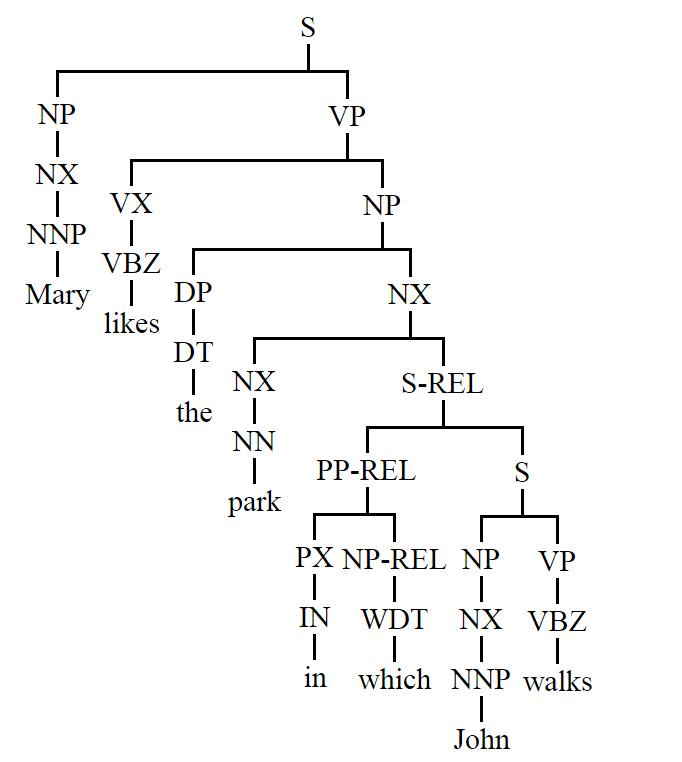
\includegraphics[scale=0.4]{EnjuParser1.png}
 	 \caption[Tree structure of a sentence]{Tree structure of a sentence}
	 \label{Figure 3}
   \end{center}
\end{figure}

\emph{\textbf{Spelling correction}} is the process in which misspelled words are corrected. Spelling correction systems are called spell checkers. Modern spell checkers (like Google's) not only correct individual misspelled words of a sentence but also have a holistic approach and try to correct the words such that the sentence as a whole becomes semantically correct. To achieve better results, spelling correctors use dictionaries and \emph{n-grams}.\\

\emph{\textbf{Word-sense disambiguation}} is the process of determining the meaning of a word. In the real world, it can happen that a word can have two or more meanings. For example, the word desert has two different meanings,a territory with sand and a dish. These "two" words, which have the same spelling, but different meanings are called homonyms.

Another linguistic phenomenon, polysemy, is when two or more words have the same spelling, and distinct and related meanings. The word "mouth" can be considered as polysemes because it can mean orifice on a face or opening of a cave or river.

Another case of word sense disambiguation are capitonyms. This is when a word has one meaning when it is capitalized, and different meaning when is not capitalized. For example the words "polish" and "Polish", which mean to make shiny and a person from Poland, respectively. \\

\emph{\textbf{Abbreviation expansion}}is the process of resolving the full expansion of an abbreviation. A system that deals with abbreviation expansions saves every pair of abbreviation and its full expansion; and then in every new occurrence of an abbreviation it refers back to the saved abbreviation and its expansion. Abbreviations in biomedical text appear often. \\

\subsection{NLP tasks which coreference resolution help}

\emph {\textbf{ Name entity recognition (NER)}} is the process in information retrieval that identifies and classifies mentions in a text that corresponds to a target group (entities) in which we are interested in. For example, in the biomedical domain we are interested in identifying proteins, genes, mutation and viruses. \\

\emph{\textbf{Relationship extraction}} is the process of identifying relations (in a text) between predefined entities. In biomedical information extraction community, the motivation of building an efficient coreference resolution system is that the community believe that coreference resolution improves accuracy of relationship extraction of biomedical entities. \\

\emph{\textbf{Machine translation}} is the process of translating a text or a speech from one language to another. These software products that translate a text from one language to another use different statistics and syntactic rules to translate one text to another. Modern machine translation systems use probabilistic models and rules to produce better translation. \\

\emph{\textbf{Question answering and natural language interfaces}} are tasks that allow humans to communicate with a computer bot. This communication is done in question and answer format. In this situation, humans ask a computer bot and the computer bot answers the humans by voice or text. In conversion (text or voice), people use pronouns and anaphoric expressions and the computer bot should resolve these anaphoric expressions. For this purpose, coreference and anaphora resolution are important components of question answering and natural language interfaces.\\

\emph{\textbf{Document summarization}}  is the process of identifying the essence of the text. This process takes a large text, as input, and return a grammatically and semantically correct smaller text, which contains the essence and the main content of the inputted text. \\

\section{Syntax}

Syntax(etymology: a Greek word syntaxis=syn [together] + taxis [arrangement]) is a discipline of linguistic, which studies the rules and patterns of ordering and connecting words in the sentence, such that the created structure of the sentence is grammatically correct.

\subsection{Words}

Words and grammatical rules are the fundamental elements to creating a grammatically correct sentence. We should be aware, that if a sentence is grammatically correct, it does not mean that it has a meaning.

These smallest units, words, are classified in different classes based on a characteristics and their function in the sentence. The main characteristic of every word is its part of speech class. Part of speech classes are divided in two subclasses: opened and closed. In the open class are: nouns (N), adjectives (ADJ), adverbs (ADV) and verbs (V). Open part of speech classes have a meaning and every open part of speech class can be extended, thus in these  classes can enter new words. In the closed set are: determiners (DET), prepositions (PREP), conjunctions (CONJ) and pronouns (PR). These part of speech classes are closed and their set of words is a fixed set.

\subsection{Phrases}

Phrase is a sequence of words, that inherits the characteristics of one of the words, which is called the head word. The phrase has a part of speech class and it inherits its part of speech class from its head word. From this characteristic, logic follows that a phrase can contain phrases and it has a recursive structure.

Other words of the phrase modify, distinguish the head object from other similar objects and give more information about the head object. These words are called modifiers.

Based on the head word, we have different type of phrases; for example noun phrases (NP) and verb phrases (VP).

\newpage
\begin{figure}[h]
   \begin{center}
	  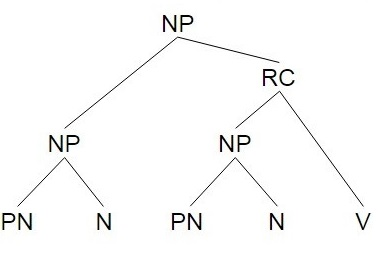
\includegraphics[scale=0.7]{nounPhraseREcursive.jpg}
 	  \caption[Recursive structure of a phrase]{Recursive structure of a phrase}
	  \label{Figure 4}
    \end{center}
\end{figure}

Phrases that their head word is a noun are called noun phrases. Usually singular noun phrases start with a singular determiner (a, an, the, this, any) or start with a proper or a common noun. Plural noun phrases start with a plural determiner (these, those, some..) or start with a plural noun. Pronouns (it, he, they, itself...) are also considered noun phrases.\\

\emph{Example (5):}
\begin{changemargin}{10mm}{10mm}
   \emph{Some rules for creating noun phrases:}
   \begin{itemize}
  	    \item \emph{\itab{ NP $\rightarrow$ N} \tab {student}}
  	    \item \emph{\itab{ NP $\rightarrow$ DET N} \tab {the student}}
  		\item \emph{\itab{ NP $\rightarrow$ DET ADJ N } \tab {the intelligent student}}
  		\item \emph{\itab{ NP $\rightarrow$ ADJ N } \tab {intelligent student}}
  		\item \emph{\itab{ NP $\rightarrow$ NP CONJ NP } \tab {a student and a professor}}
  		\item \emph{\itab{ NP $\rightarrow$ N PP } \tab {student at library}}
   \end{itemize}
\end{changemargin}
\vspace{4mm}

Phrases that their head word is a verb are called verb phrases. Verb phrases consist of a verb and are followed by a noun phrase and/or prepositional phrase. \\

\emph{Example (6):}
\begin{changemargin}{10mm}{10mm}
   \emph{  Some rules for creating verb phrases:}
    \begin{itemize}
  	    \item \emph{\itab{ VP $\rightarrow$ V} \tab {learn}}
  		\item \emph{\itab{ VP $\rightarrow$ V NP} \tab {learn history}}
  		\item \emph{\itab{ VP $\rightarrow$ V PP NP } \tab {learn at home}}
	\end{itemize}
\end{changemargin}

\vspace{4mm}

Prepositional phrases, another type of phrases in English language, consist of a preposition and a noun phrase. Prepositional phrases are used to define more specifically a noun phrase. Thus, we can say that their role is similar to adverbs and adjectives.

\subsection{Clauses}

Clauses are linguistic units that contain a noun phrase and a verb phrase. The clauses are divided into two types: dependent and independent.

\subsection{Independent clause}

An independent clause is a grammatically correct group of words that contains a noun phrase that acts as the subject of clause and a verb phrase.

The independent clause has a meaning, expresses a thought and can form alone a sentence. If a sentence has more than one clause then at least one of the clauses is independent. One of the independent clauses is main and it carries the subject and meaning of the sentence, and is called main clause.

If the sentence has two or more independent clauses they are called coordinated clauses and they are connected with a coordinating conjunction. The coordinated conjunctions are: and, but, for, nor, or, so, and yet.

Alternatively instead of a conjunction, we use a comma to connect two coordinated clauses.

\subsection{Dependent clauses}

A dependent clause is a grammatically correct group of words that contains a noun phrase (NP) and a verb phrase (VP), and it has not semantic meaning. Dependent clauses are also called subordinate clauses, because their role in the sentence is secondary. This means that if a sentence has a dependent clause, then there exist another clause that is main and independent, and the subordinate clause is dependent on the main clause. The role of subordinate clauses in the sentence is similar to adverb or adjective; they are used to describe a property, cause or a consequence of an object or a noun phrase of the main clause. Usually, the subordinate clauses are connected with the main clause or another subordinate clause with an subordinate conjunction or relative conjunction. Examples of relative conjunctions include: who, whom, that, which, what, whose; and examples of subordinate conjunctions include: although, because, if, unless, as, until, even though, even, before, when.

\subsection{Sentences}

We use sentences to express our needs, emotions, ideas, thoughts and curiosity among others. Depending what we express, we use 4 types of sentences:
\begin{itemize}
	\item declarative sentences, to make statements (.)
	\item interrogative sentences, to ask questions (?)
	\item imperative sentences, to give commands (.or !)
	\item exclamatory sentences, to express strong feelings (!)
\end{itemize}

In the biomedical articles sentences are in declarative form. Thus, I will describe the structure of the declarative sentences. In the text below, I will use the terms declarative sentence and sentence interchangeably.

A declarative sentence has at least one independent clause, and express a thought. It contains a subject (what or whom the sentence is about) and a verb (the action that the subject takes). There are cases that a sentence expresses a thought and do not contain either verb or subject. This type of sentence is called ellipsis. Ellipsis are common in dialogue. In ellipses, the speaker (writer) assumes a prior knowledge and common sense knowledge from the co-speaker (co-writer).

English language has a defined structure of the sentence and it is an ordered Subject-Verb-Object structure.This structure helps to know the position of the main parts of the sentence.

Another classification of sentences is based on the number and type of clauses that compose the sentences. These types are: simple, compound, complex and compound-complex sentences.

\emph{\textbf{Simple sentence}} consist just from one independent clause.

\emph{Example (7):}
\begin{changemargin}{10mm}{10mm}
   \emph{Proteins are assembled from amino acids.}
\end{changemargin}
\vspace{3mm}

\emph{\textbf{Compound sentences}} consists of two or more coordinated clauses connected with coordinated conjunction.\\

\emph{Example (8):}
\begin{changemargin}{10mm}{10mm}
  \emph{Bioinformatics is a science and bioinformaticians research bioinformatics.}
\end{changemargin}
\vspace{3mm}
\newpage
\emph{\textbf{Complex sentences}} consists of one independent clause and one or more subordinate clause.\\

\emph{Example (9):}
\begin{changemargin}{10mm}{10mm}
  \emph{Natural language processing is important because it helps computers to understand human language.}
\end{changemargin}
\vspace{3mm}

\emph{\textbf{Compound-complex sentences}} consists of three or more clauses, which two or more are coordinated clauses and one or more subordinate clauses.\\

\emph{Example (10):}
\begin{changemargin}{10mm}{10mm}
  \emph{Bioinformatics is a science and bioinformaticians research bioinformatics, because they want to develop mathematical models and software tools to get knowledge from biological data.}
\end{changemargin}
 \vspace{3mm}
As we can see, all these types of sentences have a specific construction. We can see that the subjects of clauses in a sentence are correlated and they tend to have same lemma, are synonyms or coreferential expressions. This construction of the sentences and this correlation between subjects of clauses helps to resolve coreference resolution.
